\section{MODULO: SISTEMA DE CONTROL DIFUSO}

\subsection{Simulación y planificación de movimiento}

Como se mencionó anteriormente el problema se puede clasificar dentro de los de planificación de movimiento (motion planning), se debe mover un objeto (robot) desde un punto inicial a un punto final evitando colisionar con los posibles obstáculos del entorno. El robot conoce su pose (el ángulo hacia dónde se orienta respecto al eje de coordenadas) en todo momento y el ángulo hacia el target, además no presenta limitaciones en cuanto al ángulo de giro. La detección de obstáculos se realiza mediante tres sensores de distancia.

Algunas consideraciones que se tuvieron en cuenta para el armado de reglas y funciones de pertenencia [6].

\begin{itemize}
    \item Cubrir adecuadamente el espacio de estado del problema.
    \item El conjunto de reglas debe ser completo y correcto.
    \item Las reglas no deben ser contradictorias.
    \item Para todos los valores de entrada la suma del grado de pertenencia de los distintos conjuntos debe ser 1.
\end{itemize}

El desarrollo de la solución se puede dividir en versiones que van desde menor a mayor complejidad. Partiendo de un ejemplo de simulación y control difuso implementado en matlab que muestra como ajustar un sistema de lógica difusa y que se puede encontrar \href{https://www.mathworks.com/help/fuzzy/tune-fuzzy-systems-using-custom-cost-function.html}{\textbf{aqui}}, a partir de ahora llamado "MySimAvoidObs1".

\subsubsection{MySimAvoidObs1}

Nuestra idea base, fue controlar con el sistema difuso la variación del ángulo actual del robot para evadir un obstáculo. En este planteo el robot no tiene información sobre el destino, solo se encarga de evadir obstáculos. De este modo se representa el control con el siguiente esquema.

\begin{center}
    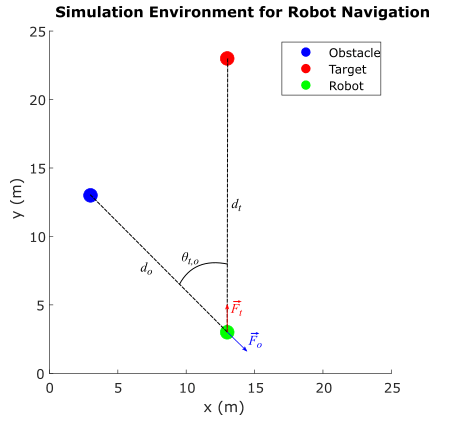
\includegraphics[scale=0.6]{Tesis/Capitulos/04_CAPITULO_2/img/MySimAvoidObs1_env.png}
    \captionof{figure}{}
\end{center}

\begin{center}
    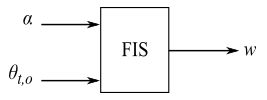
\includegraphics[scale=0.6]{Tesis/Capitulos/04_CAPITULO_2/img/MySimAvoidObs1_system.png}
    \captionof{figure}{Esquema de entradas y salidas MySimAvoidObs1.}
\end{center}

En donde $\alpha$ representa un ratio de distancia (distancia al obstáculo / distancia al target) mientras que $\theta$ la diferencia entre la dirección al target y la dirección al obstáculo.
\bigbreak
Ecuación a controlar con el sistema difuso:
\begin{equation}\boxed{
\begin{array}{rcl}
F = w*\vec{F_o} + (1-w)*\vec{F_t}
\end{array}}
\end{equation}

Tal que:
\begin{itemize}
    \item $\vec{F_t}$ Vector al target.
    \item $\vec{F_o}$ Vector contrario al obstáculo.
    \item w: Parámetro [0-1].
\end{itemize}

De esta manera, a continuación en la imagen \ref{fig:MySymAvoidObs1} se puede ver como la composición de fuerzas ayuda al sistema de control a evitar colisionar con el obstáculo.

\begin{center}
    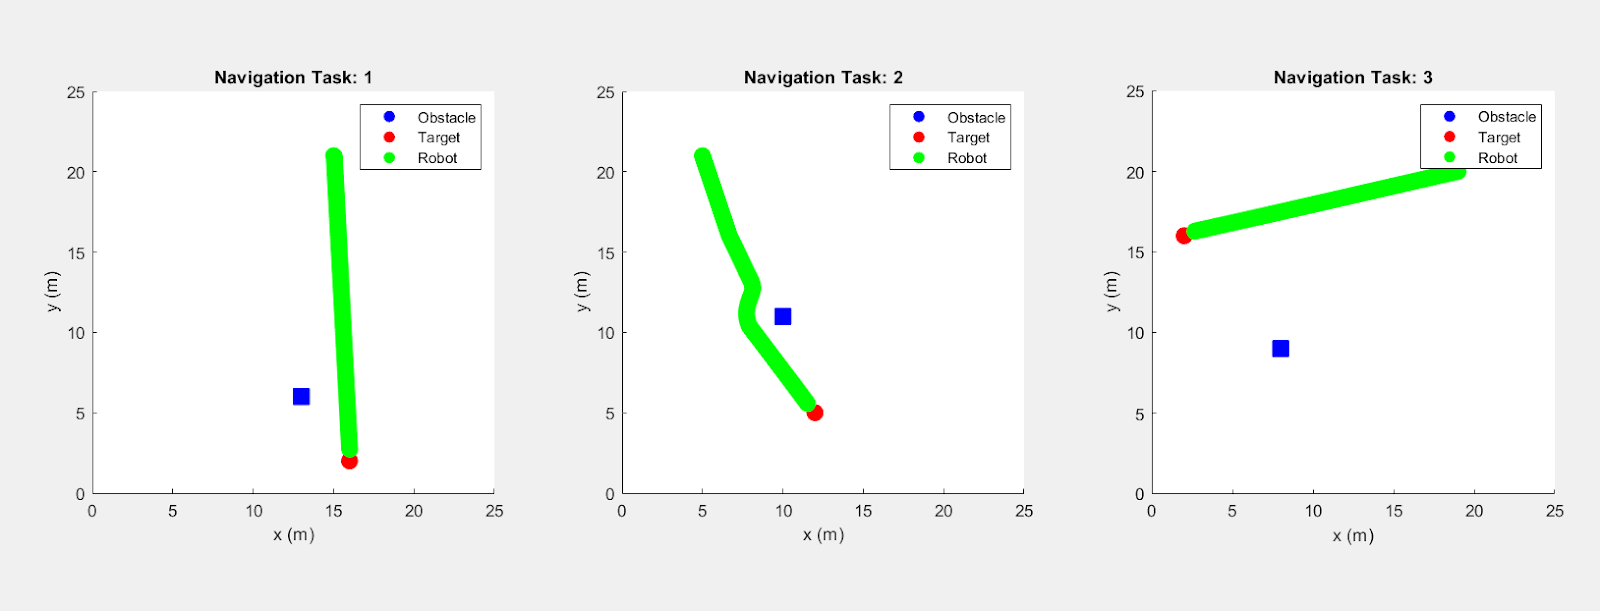
\includegraphics[scale=0.3]{Tesis/Capitulos/04_CAPITULO_2/img/MySimAvoidObs1.png}
    \captionof{figure}{Captura de la simulacion de MySimAvoidObs2.}
    \label{fig:MySymAvoidObs1}
\end{center}

Esta simulación no fue la que se llevo a la practica ya que para saber todo el tiempo donde se encuentra el obstáculo es necesario tener múltiples sensores al rededor del robot, como muestra la figura \ref{fig:MySymAvoidObs1ms} .\par

\begin{center}
    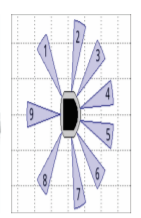
\includegraphics[width=5cm, height=5cm]{Tesis/Capitulos/04_CAPITULO_2/img/robot_multiple_sensors.png}
    \captionof{figure}{Robot con multiples sensores.}
    \label{fig:MySymAvoidObs1ms}
\end{center}

\subsubsection{MySimAvoidObs2}

En esta versión proponemos un nuevo sistema de control difuso el cual únicamente necesite utilizar tres sensores de distancia.

\begin{center}
    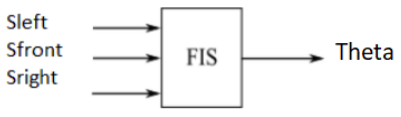
\includegraphics[scale=0.5]{Tesis/Capitulos/04_CAPITULO_2/img/esquema1.png}
    \captionof{figure}{Esquema de entradas y salidas MySimAvoidObs2.}
\end{center}

En donde Sleft, Sfront, y Sright representa las distancias al obstáculo y Theta el ángulo que deberá girar el robot para evadirlo.

Ecuación a controlar con el sistema difuso:
\begin{equation}\boxed{
\begin{array}{rcl}
nav.robot(3) = nav.robot(3) - Theta;
\end{array}}
\end{equation}

Tal que:
\begin{itemize}
    \item nav.robot(3) representa la dirección de avance actual del robot.
    \item Theta la salida del sistema difuso, evasión del obstáculo.
\end{itemize}

A continuación en la imagen \ref{fig:MySymAvoidObs2_1} del simulador y sus recorridos se puede observar como el vehículo parte de un punto de inicio (circulo amarillo) y es capaz de pasar a lo largo de todo el sendero de obstáculos evitando colisionar. 

\begin{center}
    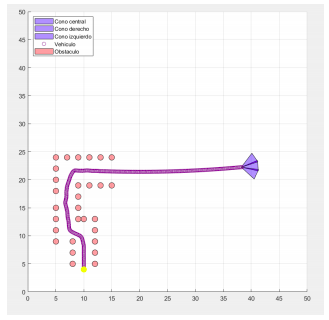
\includegraphics[scale=0.5]{Tesis/Capitulos/04_CAPITULO_2/img/res_1.png}
    \captionof{figure}{MySimAvoidObs2}
    \label{fig:MySymAvoidObs2_1}
\end{center}

\subsubsection{MySimReachTarget}

En esta versión la tarea de navegación se trata de combinar dos vectores, la variación del ángulo actual (ángulo que proporciona una dirección libre de colisión para el robot) y el ángulo al target. La salida w varía entre 0 y 1 e indica el peso que tendrá cada ángulo en el ángulo resultado tal como se muestra en la ecuación de control. Es una combinación de los sistemas implementados en las versiones anteriores "MySimAvoidObs1" y "MySimAvoidObs2".


\begin{center}
    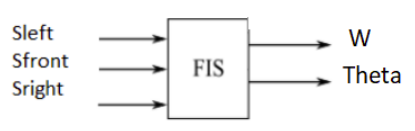
\includegraphics[scale=0.5]{Tesis/Capitulos/04_CAPITULO_2/img/esquema2.png}
    \captionof{figure}{Esquema de entradas y salidas MySimReachTarget.}
\end{center}

Ecuación a controlar con el sistema difuso:

\begin{equation}\boxed{
\begin{array}{rcl}
nav.robot(3)=(1-w)(nav.robot(3)-Theta) + w(ang);
\end{array}}
\end{equation}

Tal que:

\begin{itemize}
    \item nav.robot(3) representa la dirección de avance actual del robot.
    \item Theta la salida del sistema difuso, evasión del obstáculo.
    \item w: Parámetro [0-1].
    \item ang: ángulo al target con respecto a la horizontal en cada ubicación del robot.
\end{itemize}

A continuación en las imágenes \ref{fig:MySimReachTarget_1} y \ref{fig:MySimReachTarget_2} se puede observar como en este caso el robot es capaz no solo de evadir los obstáculos a los cuales se enfrenta si no también tiene la capacidad de alcanzar un punto especificado como target (circulo rojo).

\begin{figure}[ht]
\centering
\subfigure[MySimAvoidObs2]{
\begin{minipage}[ht]{0.25\linewidth}
\centering
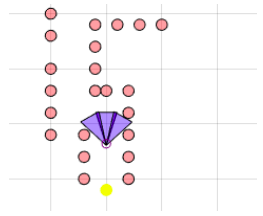
\includegraphics[width=2in]{Tesis/Capitulos/04_CAPITULO_2/img/des1.png}
\label{fig:MySimReachTarget_1}
\end{minipage}%
}
\subfigure[MySimAvoidObs2]{
\begin{minipage}[ht]{0.25\linewidth}
\centering
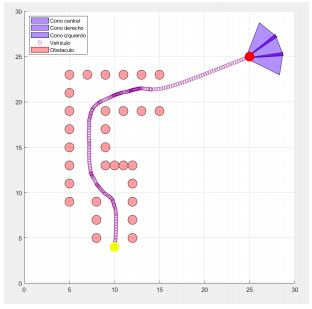
\includegraphics[width=2in]{Tesis/Capitulos/04_CAPITULO_2/img/res_2.png}
\label{fig:MySimReachTarget_2}
\end{minipage}%
}
\end{figure}

\subsubsection{MySimReachTargetVelControl}

En la cuarta versión la ecuación de control se mantiene igual, pero se agrega a la como salida del control difuso el control de la velocidad del robot, permitiéndole así ser capaz de controlar su velocidad.

\begin{center}
    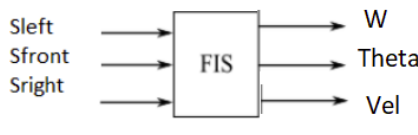
\includegraphics[scale=0.5]{Tesis/Capitulos/04_CAPITULO_2/img/esquema4.png}
    \captionof{figure}{Esquema de entradas y salidas MySimReachTarget.}
\end{center}

\begin{equation}\boxed{
\begin{array}{rcl}
nav.robot(3)=(1-w)(nav.robot(3)-Theta) + w(ang);
\end{array}}
\end{equation}

\subsubsection{Variables Fuzzy}

A continuación se muestra el detalle de las funciones de pertenencia de las variables intervinientes en el control difuso. 
Consideramos como entradas la distancia al obstáculo obtenida mediante tres sensores con ángulo ajustable. En los tres sensores se repiten las funciones “cerca” y “lejos”.\par

\begin{center}
    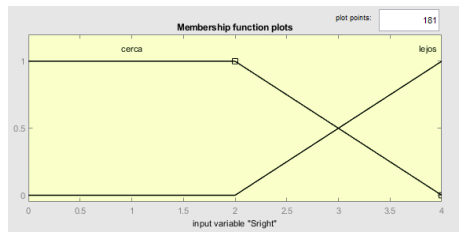
\includegraphics[scale=0.5]{Tesis/Capitulos/04_CAPITULO_2/img/varfuzzy1.png}
    \captionof{figure}{Detalle de funciones de pertenencia de entrada Sright, sensor derecho de distancia.}
\end{center}

Para la salida Theta definimos las funciones “izquierda” “centro” y “derecha”, recordamos que Theta hace referencia al ángulo necesario que deberá tomar el robot para evadir el obstáculo que tenga enfrente.

\begin{center}
    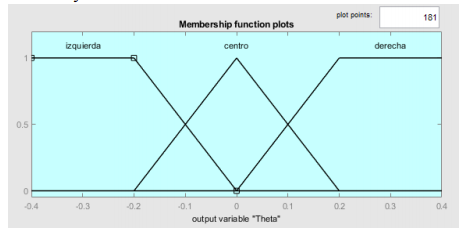
\includegraphics[scale=0.5]{Tesis/Capitulos/04_CAPITULO_2/img/varfuzzy2.png}
    \captionof{figure}{Detalle de funciones de pertenencia de salida Theta.}
\end{center}

Para la salida w se definieron los conjuntos “bajo” y “alto” según la prioridad que le dará el robot alcanzar el target o evadir el obstáculo cercano.

\begin{center}
    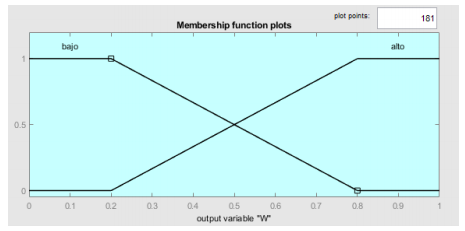
\includegraphics[scale=0.5]{Tesis/Capitulos/04_CAPITULO_2/img/varfuzzy3.png}
    \captionof{figure}{Detalle de funciones de pertenencia de salida w.}
\end{center}

Finalmente la variable de salida "Vel" permite que el robot modifique la velocidad según la ubicación de los obstáculos. Se definieron las funciones “LENTO”, “MEDIO” y “RAPIDO”. 

AGREGAR FOTO ACA!!!!!!!

El esquema del control difuso de la última versión con estas entradas y salidas se muestra en la figura \ref{fig:esquema}.

\begin{center}
    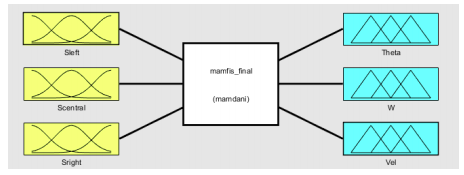
\includegraphics[scale=0.5]{Tesis/Capitulos/04_CAPITULO_2/img/varfuzzy4.png}
    \captionof{figure}{Sistema de control difuso de MySimReachTargetVelControl.}
    \label{fig:esquema}
\end{center}

\subsubsection{Sets de reglas}


\subsection{Implementación en C del sistema de control difuso}